\begin{definition}[Almost Disjoint Intervals] \leavevmode\\
    We say two intervals $I$ and $J$ are almost disjoint if either $I\cap J= \emptyset$ or $I\cap J$ has a single element.
\end{definition}

\begin{definition}[Partition] \leavevmode\\
    \begin{description}
        \item[First Viewpoint: ] A partition $P$ of an interval $[a,b]$ is a finite set of points in $[a,b]$ that include both $a$ and $b$. We always list the points of a partition $P=\{x_0, ..., x_n\}$ in increasing order:
        $$
            x_0 = a < x_1 < x_2 < ... < b = x_n
        $$
        \item[Second Viewpoint: ] A partition $P$ of an interval $[a,b]$ is a finite collection of almost disjoint (nonempty) compact intervals whose union is $[a,b]$:
        $$
        P = {I_1,..., I_n} \text{ where } I_1=[x_0, x_1], I_2=[x_1,x_2], ..., I_n = [x_{n-1}, x_n] ~~(\text{with }x_0 = a, x_1 = b)
        $$
    \end{description}
    
\end{definition}

\begin{example}
    \begin{align*}
        P = \left\{0, \frac{1}{5}, \frac{1}{2}, \frac{5}{6}, 1\right\} \\
        P = \left\{[0, \frac{1}{5}], [\frac{1}{5}, \frac{1}{2}], [\frac{1}{2}, \frac{5}{6}], [\frac{5}{6}, 1]\right\}
    \end{align*} are both partitions of $[0,1]$.
\end{example}

\begin{figure}[h]
    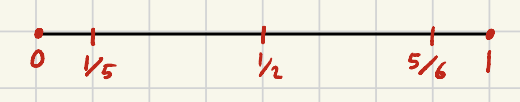
\includegraphics[width=.50\linewidth, center]{/Users/josiahvillarante/GradSchool/Grad-School-Notes/Math230B/Lecture/CH6/images/Partition 1.png}
\end{figure}

\begin{notation}
Let $f:[a,b] \to \R$ be a bounded function. Let $P = \left\{x_0 = a, ..., x_n = b\right\}$ be a partition of $[a,b]$. We let
\begin{align*}
    &m = \inf \left\{f(x) : x \in [a,b]\right\} \\
    &M = \sup \left\{f(x) : x \in [a,b]\right\} \\
    \forall 1 \leq k \leq n ~~&m_k = \inf \left\{f(x) : x \in [x_{k-1}, x_k]\right\} \\
    \forall 1 \leq k \leq n ~~&M_k = \sup \left\{f(x) : x \in [x_{k-1}, x_k]\right\}
\end{align*}
The existence of $m, M, m_k, M_k$ as real numbers is guaranteed due to the assumption that $f$ is bounded on $[a,b]$.
\end{notation}

\begin{remark}
    Suppose $A$ and $B$ are nonempty, bounded sets in $\R \st A \subseteq B$. Then 
    \begin{enumerate}[$(i)$]
        \item $\inf A \leq \sup A$
        \item $\inf B \leq \sup B$
        \item $\sup A \leq \sup B$
        \item $\inf A \geq \inf B$
    \end{enumerate}
    As a result
    $$
    \forall 1 \leq k \leq n ~~m \leq m_k \leq M_k \leq M
    $$
\end{remark}

\begin{remark}
    If $f: [a,b] \to \R$ is continuous, then $f$ attains its maximum and minimum over each compact subinterval. In this case,
    \begin{align*}
        m_k &= \min \left\{f(x) : x \in [x_{k-1}, x_k]\right\} \\
        M_k &= \max \left\{f(x) : x \in [x_{k-1}, x_k]\right\}
    \end{align*}
\end{remark}

\begin{definition}[Lower Sum, Upper Sum]\leavevmode\\
    Let $f: [a,b] \to \R$ be bounded and let $\alpha: [a,b] \to \R$ be increasing. Let $P=\{x_0, ..., x_n\}$ be a partition of $[a,b]$. Let $\Delta_{\alpha_k}=\alpha(x_k) - \alpha(x_{k-1})$.
    \begin{enumerate}[$(i)$]
        \item The lower Riemann-Stieltjes sum of $f$ (R.S. sum of $f$) with respect to $\alpha$ for the partition $P$ is defined by
        $$
        L(f, \alpha, P) = \sum_{k=1}^{n}m_k \left(\alpha(x_k)-\alpha(x_{k-1})\right) = \sum_{k=1}^{n}m_k \Delta \alpha_k
        $$
        \item The upper Riemann-Stieltjes sum of $f$ (R.S sum of $f$) with respect $\alpha$ for the partition $P$ is defined by 
        $$
        U(f, \alpha, P) = \sum_{k=1}^{n}M_k \left(\RSdeltadiff{k}{k-1}\right) = \RSupsum
        $$
    \end{enumerate}
\end{definition}

\begin{note}
    Note that
    $$
    m(\alpha(b)-\alpha(a)) \leq L(f, \alpha, P) \leq U(f, \alpha, P) \leq M(\alpha(b) - \alpha(a))
    $$
    Indeed,
    \begin{align*}
        L(f, \alpha, P) = \RSlowsum &\geq \sum_{k=1}^{n} m (\RSdeltadiff{k}{k-1}) \\
        &= m \sum_{k=1}^{n} \RSdeltadiff{k}{k-1} \\
        &= m \left[\RSdeltadiff{1}{0} + \RSdeltadiff{2}{1} +... + \RSdeltadiff{n}{n-1}\right] \\
        &= m \left[\RSdeltadiff{n}{0}\right] \\ 
        &= m \left[\alpha(b) - \alpha(a)\right]
    \end{align*}
    Similarly,
    \begin{align*}
        U(f, \alpha, P) = \RSupsum &\leq \sum_{k=1}^{n} M (\RSdeltadiff{k}{k-1}) \\
        &= M \sum_{k=1}^{n} \RSdeltadiff{k}{k-1} \\
        &= M \left[\RSdeltadiff{1}{0} + \RSdeltadiff{2}{1} +... + \RSdeltadiff{n}{n-1}\right] \\
        &= M \left[\RSdeltadiff{n}{0}\right] \\ 
        &= M \left[\alpha(b) - \alpha(a)\right]
    \end{align*}
\end{note}

\begin{notation}
    $\Pi [a,b]$, or $\Pi$ for short, denotes the collection of all the possible partitions of $[a,b]$.
\end{notation}

\begin{definition}[Upper Riemann-Stieltjes Integral, Lower Riemann-Stieltjes Integral] \leavevmode\\
    Let $f:[a,b] \to \R$ be bounded and $\alpha : [a,b] \to \R$ be increasing.
    \begin{enumerate}[$(i)$]
        \item The upper Riemann-Stieltjes integral of $f$ with respect to $\alpha$ (on $[a,b]$) is defined by 
        $$
        U(f, \alpha) = \UpperInt{f} = \inf \{U(f, \alpha, P) : P \in \Pi \}
        $$
        (Note that the set $\{U(f, \alpha, P) : P \in \Pi\}$ of all upper sums is bounded below by $m(\alpha(b) - \alpha(a))$, so the infimum is a real number)
        
        \item The lower Riemann-Stieltjes integral of $f$ with respect to $\alpha$ (on $[a,b]$) is defined by 
        $$
        L(f, \alpha) = \LowerInt{f} = \sup \{L(f, \alpha, P) : P \in \Pi\}
        $$
    \end{enumerate}
\end{definition}

\begin{definition} [Riemann-Stieltjes Integrable Function] \leavevmode\\
    Let $\alpha : [a,b] \to \R$ be an increasing function. A function $f: [a,b] \to \R$ is said to be Riemann-Stieltjes integrable (on $[a,b]$) with respect to $\alpha$ if 
    \begin{enumerate}[$(i)$]
        \item $f$ is bounded
        \item $L(f, \alpha) = U(f, \alpha)$
    \end{enumerate}
    In this case, the Riemann-Stieltjes integral of $f$ with respect to $\alpha$, denoted by
    $$
    \text{$\int_{a}^{b}f d\alpha$ or $\int_{a}^{b}f(x) d\alpha$ or $\int_{[a,b]}fd\alpha$}
    $$
    is the common value of $L(f, \alpha)$ and $U(f, \alpha)$. That is,
    $$
    \int_{a}^{b}f d\alpha = L(f, \alpha) = U(f, \alpha)
    $$
\end{definition}

\begin{example}
    Let $c$ be a fixed real number. Prove that the constant function $f(x) = c$ on $[a,b]$ is R.S. integrable and
    $$
    \int_{a}^{b}f d\alpha = c (b-a)
    $$
\end{example}
\begin{proof}
    For any partition $P = \{x_0, ..., x_n\}$ of $[a,b]$ we have
    \begin{align*}
        \forall 1 \leq k \leq n &m_k = \inf\{f(x) : x \in [x_{k-1}, x_k]\} = \inf \{c\} = c \\
        &M_k = \sup\{f(x) : x \in [x_{k-1}, x_k]\} = \sup \{c\} = c
    \end{align*}
    Therefore,
    \begin{align*}
        L(f, \alpha, P) &= \sum_{k=1}^{n}m_k (\RSdeltadiff{k}{k-1}) \\
        &= \sum_{k=1}^{n}c (\RSdeltadiff{k}{k-1}) \\
        &= c \sum_{k=1}^{n} \RSdeltadiff{k}{k-1} \\
        &= c [\alpha(b) - \alpha(a)]
    \end{align*}
    and
    \begin{align*}
        U(f, \alpha, P) &= \sum_{k=1}^{n}M_k (\RSdeltadiff{k}{k-1}) \\
        &= \sum_{k=1}^{n}c (\RSdeltadiff{k}{k-1}) \\
        &= c \sum_{k=1}^{n} \RSdeltadiff{k}{k-1} \\
        &= c [\alpha(b) - \alpha(a)]
    \end{align*}
    Hence,
    \begin{align*}
        L(f, \alpha) = \sup \{L(f, \alpha, P) : P \in \Pi\} = \sup \{c (\alpha(b) - \alpha(a))\} = c(\alpha(b) - \alpha(a)) \\
        U(f, \alpha) = \inf \{U(f, \alpha, P) : P \in \Pi\} = \inf \{c(\alpha(b) - \alpha(a))\} = c(\alpha(b) - \alpha(a))
    \end{align*}
    Since $L(f, \alpha) = U(f, \alpha) = c(\alpha(b) - \alpha(a))$, we conclude that $f$ is R.S. integrable with respect to $\alpha$ and 
    $$
    \int_{a}^{b} f d\alpha = c[\alpha(b) - \alpha(a)]
    $$
    \qed
\end{proof}

\begin{example}
    Let $f:[a,b] \to \R$ be bounded and let $\alpha : [a,b] \to \R$ be a constant function ($\alpha (x) = c$). Prove that $\int_{a}^{b}f d\alpha = 0.$
\end{example}
\begin{proof}
    For any partition $P= \{x_0, ..., x_n\}$ of $[a,b]$,
    \begin{align*}
        L(f, \alpha, P) = \sum_{k=1}^{n}m_k \left[\RSdeltadiff{k}{k-1}\right] = \sum_{k=1}^{n}m_k \cdot 0 =0 \\ 
        U(f, \alpha, P) = \sum_{k=1}^{n}M_k \left[\RSdeltadiff{k}{k-1}\right] = \sum_{k=1}^{n}M_k \cdot 0=0
    \end{align*}
    Therefore,
    \begin{align*}
        L(f, \alpha) = \sup \{L(f, \alpha, P) : P \in \Pi\} = 0 \\
        U(f, \alpha) = \inf \{U(f, \alpha, P) : P \in \Pi\} = 0
    \end{align*}
    So $L(f, \alpha) = U(f, \alpha) = 0 \implies \int_{a}^{b}f d\alpha = 0.$
    \qed
\end{proof}

\begin{example}
    Let $f: [a,b] \to \R$ be defined by
    $$
    f(x) = \begin{cases*}
        1 &if $x \in \Q$ \\
        0 &if $x \not \in \Q$
    \end{cases*}
    $$
    Prove that
    \begin{enumerate}[$(i)$]
        \item if $\alpha : [a,b] \to \R$ is constant, then $\int_{a}^{b}f d\alpha = 0$ (proved in the last example)
        \item if $\alpha : [a,b] \to \R$ is increasing and $\alpha(a) \not = \alpha(b)$, then $f \not \in R_{\alpha}[a,b]$
    \end{enumerate}
\end{example}

\begin{proof}
$(ii)$ For any partition $P=\{x_0, ..., x_n\}$ of $[a,b]$ we have
    \begin{align*}
        \forall 1 \leq k \leq n ~~~&m_k = \inf \{f(x) : x\in [x_{k-1}, x_k]\} = \inf \{0,1\} = 0 \\ 
        &M_k = \sup \{f(x) : x \in [x_{k-1}, x_k]\} = \sup \{0,1\} = 1
    \end{align*}
    Therefore
    \begin{align*}
        L(f, \alpha, P) &= \sum_{k=1}^{n}m_k \left[\RSdeltadiff{k}{k-1}\right] = 0 \cdot \left[\alpha(b) - \alpha(a)\right] = 0 \\
        U(f, \alpha, P) &= \sum_{k=1}^{n}M_k \left[\RSdeltadiff{k}{k-1}\right] = 1 \cdot \left[\alpha(b) - \alpha(a)\right] = \alpha(b) - \alpha(a)
    \end{align*}
    Hence
    $$
    \begin{rcases*}
        L(f, \alpha) = \sup \{L(f, \alpha, P) : P \in \Pi\} = 0 \\
        U(f, \alpha) = \inf \{U(f, \alpha, P) : P \in \Pi\} = \alpha(b) - \alpha(a)
    \end{rcases*} \implies L(f, \alpha) \not = U(f, \alpha) \implies f \not \in R_{\alpha}[a,b]
    $$
    \qed
\end{proof}

\begin{definition}[Refinement of a Partition] \leavevmode\\
    \begin{description}
        \item[First Viewpoint: ] A partition $Q = \{z_0, ..., z_m\}$ of $[a,b]$ is a refinement of a partition $P=\{x_0, ..., x_n\}$ of $[a,b]$ if $P \subseteq Q$. That is, if $Q$ contains all points of $P$.
        \item[Second Viewpoint: ] A partition $Q={J_1, ..., J_m}$ of $[a,b]$ is a refinement of a partition $P=\{I_0, ..., I_n\}$ of $[a,b]$ if every interval $I_k$ of $P$ is an almost disjoint union of one or more intervals of $Q$.  
    \end{description}
\end{definition}

\begin{example}
    Consider the following partitions of $[0,1]$:
    \begin{align*}
        P &= \{0, \frac{1}{2}, 1\} \\
        Q &= \{0, \frac{1}{3}, \frac{1}{2}, 1\}
    \end{align*}
    Then $Q$ is a refinement of $P$ since $P \subseteq Q$.
\end{example}

\begin{remark}
    Let $P$ and $Q$ be any two partitions of $[a,b]$. Then $P \cup Q$ will be a refinement of both $P$ and $Q$ because $P \subseteq P \cup Q$ and $Q \subseteq P \cup Q$. So, any two partitions of $[a,b]$ have a common refinement.
\end{remark}

\begin{example}
    Consider the following partitions of $[0,1]$:
    \begin{align*}
        P&=\{0, \frac{1}{2}, 1\} \\
        Q&= \{0, \frac{1}{3}, \frac{2}{3}, 1\}
    \end{align*}
    $P$ is not a refinement of $Q$ and $Q$ is not a refinement of $P$, but 
    $$
    P\cup Q = \{0, \frac{1}{3}, \frac{1}{2}, \frac{2}{3}, 1\}
    $$
    is a refinement of both $P$ and $Q$.
\end{example}

\begin{definition}[Size of a Partition] \leavevmode\\
    Let $P=\{x_0, ..., x_n\}$ be a partition of $[a,b]$. The size of $P$, denoted $||P||$, is defined by 
    \begin{align*}
        ||P|| &= \max \left\{|x_k - x_{k-1}| : 1 \leq k \leq n\right\} \\
        &= \max \left\{|x_1 - x_0|, |x_2 - x_1|, ..., |x_n - x_{n-1}|\right\}
    \end{align*}
\end{definition}